\documentclass{article}
\newcommand{\mydate}{November 3, 2025}
\newcommand{\mytitle}{QM HW7}
\title{\textbf{\mytitle}}
\author{Jiete XUE}
\date{\mydate}
\usepackage{fancyhdr}
\pagestyle{fancy}
\fancyhf{}
\fancyhead[C]{\mytitle }
\fancyhead[R]{Jiete Xue}
\fancyhead[L]{\mydate}
\fancyfoot[C]{\thepage}
\usepackage{amsthm}
\usepackage{amsmath}
\usepackage{amssymb}
\usepackage{physics}
\usepackage{tikz}
\usepackage{float}

%% 右矢
%\ket{\psi}          % 输出:|ψ⟩
%\ket{\psi(t)}       % 输出:|ψ(t)⟩
%
%% 左矢
%\bra{\phi}          % 输出:⟨φ|
%
%% 期望值
%\expval{\hat{A}}    % 输出:⟨Â⟩
%\expval{\hat{A}}{\psi}  % 输出:⟨ψ|Â|ψ⟩
%
%% 对易子
%\comm{\hat{A}}{\hat{B}}  % 输出:[Â, B̂]
\newtheoremstyle{1}{}{}{}{}{\bfseries}{}{\newline}{}
\theoremstyle{1}
\newtheorem{problem}{Problem}
\usepackage{chngcntr}
\counterwithin{equation}{problem}
\newcommand{\pa}{\partial}
\newcommand{\rn}[1]{\romannumeral #1\relax}
\newcommand{\Rn}[1]{\expandafter\@slowromancap\romannumeral#1@}
\newcommand{\ii}{\mathrm{i}}
\newcommand{\ee}{\mathrm{e}}

\begin{document}
\maketitle
\begin{problem}[Hydrogen atom wavefunction]
(1) 
\begin{equation}
    \psi_{n_r,l,m}=R_{n_r,l}(r)Y_{l}^m(\theta,\phi),
\end{equation}
where, $Y_l^m$ is the spherical harmonics and 
\begin{equation}
    R_{n_R,l}(r)\sim \rho^l \ee^{-\frac{\rho}{2}}L_{n_r}^{2l+1}(\rho),
\end{equation}
\begin{equation}
    \rho=\frac{2r}{na_0},\ a_0 =\frac{4\pi\epsilon_0 \hbar^2}{m_e e^2}\text{is a constant.}
\end{equation}
\begin{equation}
    E_n=\frac{E_0}{n^2}.
\end{equation}
(2) 
\begin{equation}
    \psi_{100}(r,\theta,\phi) = \frac{1}{\sqrt{\pi a_0^3}} \, e^{-r/a_0}
\end{equation}
\begin{equation}
    \psi_{200}(r,\theta,\phi) = \frac{1}{\sqrt{32\pi a_0^3}} \left( 2 - \frac{r}{a_0} \right) e^{-r/(2a_0)}
\end{equation}
\begin{equation}
    \psi_{210}(r,\theta,\phi) = \frac{1}{\sqrt{32\pi a_0^3}} \frac{r}{a_0} e^{-r/(2a_0)} \cos\theta
\end{equation}
\begin{equation}
    \psi_{21\pm1}(r,\theta,\phi) = \frac{1}{\sqrt{64\pi a_0^3}} \frac{r}{a_0} e^{-r/(2a_0)} \sin\theta \, e^{\pm i\phi}
\end{equation}
\begin{equation}
    \psi_{300}(r,\theta,\phi) = \frac{1}{81\sqrt{3\pi a_0^3}} \left( 27 - 18\frac{r}{a_0} + 2\frac{r^2}{a_0^2} \right) e^{-r/(3a_0)}
\end{equation}
\begin{equation}
    \psi_{310}(r,\theta,\phi) = \frac{\sqrt{2}}{81\sqrt{\pi a_0^3}} \left( 6 - \frac{r}{a_0} \right) \frac{r}{a_0} e^{-r/(3a_0)} \cos\theta
\end{equation}
\begin{equation}
    \psi_{31\pm1}(r,\theta,\phi) = \frac{1}{81\sqrt{\pi a_0^3}} \left( 6 - \frac{r}{a_0} \right) \frac{r}{a_0} e^{-r/(3a_0)} \sin\theta \, e^{\pm i\phi}
\end{equation}
\begin{equation}
    \psi_{320}(r,\theta,\phi) = \frac{1}{81\sqrt{6\pi a_0^3}} \frac{r^2}{a_0^2} e^{-r/(3a_0)} (3\cos^2\theta - 1)
\end{equation}
\begin{equation}
    \psi_{32\pm1}(r,\theta,\phi) = \frac{1}{81\sqrt{\pi a_0^3}} \frac{r^2}{a_0^2} e^{-r/(3a_0)} \sin\theta\cos\theta \, e^{\pm i\phi}
\end{equation}
\begin{equation}
    \psi_{32\pm2}(r,\theta,\phi) = \frac{1}{162\sqrt{\pi a_0^3}} \frac{r^2}{a_0^2} e^{-r/(3a_0)} \sin^2\theta \, e^{\pm 2i\phi}
\end{equation}
When $l>0$, $r^l$ tend to $0$ with $r$ tend to $0$. When $l=0$, value at $r=0$ is not $0$ with a non-zero derivative. So cusps appear when $l=0$.

\end{problem}
\begin{problem}[Gaussian orbital approximation]
    (1) 
    \begin{equation}
        \psi_{1s}(\mathbf{r})=\frac{1}{\sqrt{\pi a^3}}\ee^{-\frac{r}{a}},\ \psi_{1s}^G(\mathbf{r})=\sqrt{\frac{2\sqrt{2}}{\pi^\frac{3}{2}\lambda^3}}\ee^{-\frac{r^2}{\lambda^2}}.
    \end{equation}
    \begin{equation}
    \begin{aligned}
            \mathrm{Err}(\lambda)&=4\pi\int_{0}^{+\infty}\left|\frac{1}{\sqrt{\pi a^3}}\ee^{-\frac{r}{a}}-\sqrt{\frac{2\sqrt{2}}{\pi^\frac{3}{2}\lambda^3}}\ee^{-\frac{r^2}{\lambda^2}}\right|^2 r^2\dd{r}\\
            &=2-\sqrt{\frac{128\sqrt{2}}{\sqrt{\pi}a^3\lambda^3}}\ee^{\left(\frac{\lambda}{2a}\right)^2}\int_{0}^{+\infty}\ee^{-\left(\frac{r}{\lambda}+\frac{\lambda}{2a}\right)^2}r^2\dd{r}.
    \end{aligned}
    \end{equation}
    Let $\lambda=k a$, then 
    \begin{equation}
        \mathrm{Err}=2-8\sqrt{2}\left(\frac{2}{\pi}\right)^{1/4}k^{\frac{3}{2}}\ee^{\left(\frac{k}{2}\right)^2}\int_{0}^{+\infty}\ee^{-\left(x+\frac{k}{2}\right)^2}x^2\dd{x}.
    \end{equation}
    We require 
    \begin{equation}
        \frac{\pa \ln \mathrm{Err}}{\pa k}=0,
    \end{equation}
    \begin{equation}
        \frac{3}{2k}+\frac{k}{2}-\frac{\int_{0}^{+\infty}\left(x+\frac{k}{2}\right)\ee^{-\left(x+\frac{k}{2}\right)^2}x^2\dd{x}}{\int_{0}^{+\infty}\ee^{-\left(x+\frac{k}{2}\right)^2}x^2\dd{x}}=0.
    \end{equation}
    \begin{figure}[H]
        \centering
        \includegraphics[width=0.8\textwidth]{s-orbit-k.png}
        \caption{The relation between $k$ and the LHS of the equation of 1s orbit.}
    \end{figure}
    We can get the value of $k$ is about $1.92$. (But AI said it is about $1.34$, and $k=1.92$ let $\mathrm{Err}<0$.)
    $$^\divideontimes \ _{-} \ ^\divideontimes ?$$
    (2)\begin{equation}
        \psi_{2p_z}=\frac{1}{\sqrt{32 \pi a^5}}r \cos \theta  \ee^{-\frac{r}{2a}}.
    \end{equation}
    \begin{equation}
        \psi_{2p_z}^G=\sqrt{\frac{8 \sqrt{2}}{\pi^{\frac{3}{2}}\lambda^5}}r\cos \theta \ee ^{-\frac{r^2}{\lambda^2}}.
    \end{equation}
    The exponent part is similar to (1). So we want to find the extreme point of
    \begin{equation}
        \left(\frac{k}{4}\right)^2+\frac{5}{2}\ln k+\ln \int_{0}^{+\infty}\ee^{-(x+k/4)^2}x^4\dd{x}.
    \end{equation}
    \begin{figure}[H]
        \centering
        \includegraphics[width=0.8\textwidth]{p-orbit-k.png}
        \caption{The relation between $k$ and the LHS of the equation of 2p orbit.}
    \end{figure}
    $k\approx 4.77$
    \newline
    (3) 



    \tikzset{every picture/.style={line width=0.75pt}} %set default line width to 0.75pt        
    \begin{center}
        
        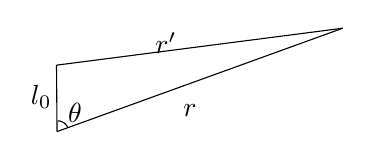
\begin{tikzpicture}[x=0.75pt,y=0.75pt,yscale=-0.5,xscale=0.5]
        %uncomment if require: \path (0,300); %set diagram left start at 0, and has height of 300
        
        %Straight Lines [id:da08410565510102352] 
        \draw    (219.25,144.5) -- (219.75,208.5) ;
        %Straight Lines [id:da804324153630842] 
        \draw    (219.75,208.5) -- (495.04,108.9) ;
        %Shape: Arc [id:dp6152558653728653] 
        \draw  [draw opacity=0] (220.26,198.01) .. controls (224.54,198.19) and (228.2,200.6) .. (229.93,204.03) -- (219.75,208.5) -- cycle ; \draw   (220.26,198.01) .. controls (224.54,198.19) and (228.2,200.6) .. (229.93,204.03) ;  
        %Straight Lines [id:da9942608069256513] 
        \draw    (219.25,144.5) -- (495.04,108.9) ;
        
        % Text Node
        \draw (228,178.4) node [anchor=north west][inner sep=0.75pt]    {$\theta $};
        % Text Node
        \draw (339,180.4) node [anchor=north west][inner sep=0.75pt]    {$r$};
        % Text Node
        \draw (192,161.4) node [anchor=north west][inner sep=0.75pt]    {$l_{0}$};
        % Text Node
        \draw (312,110.4) node [anchor=north west][inner sep=0.75pt]    {$r'$};
        
        
        \end{tikzpicture}
        \end{center}
        \begin{equation}
            r'^2=r^2-2 rl_0\cos \theta +l_0^2.
        \end{equation}
        \begin{equation}
            \begin{aligned}
                &\int \dd{\mathbf{r}} \psi^{G*}_{1s}(\mathbf{r})\psi_{1s}^G(\mathbf{r}-l_0\hat{\mathbf{z}})\\
                =&\frac{4\sqrt{2}}{\sqrt{\pi}\lambda^3}\int_{(r,\theta)\in \left[0,+\infty\right]\times \left[0,\pi\right]}\exp\left[-\frac{2r^2-2rl_0\cos\theta+l_0^2}{\lambda^2}\right]r^2\sin\theta\dd{r}\dd{\theta}\\
                =&\frac{4\sqrt{2}}{\sqrt{\pi}\lambda^3} \int_{0}^{+\infty}\left[\ee^{-2\left(r-l_0/2\right)^2/\lambda^2}-\ee^{-2\left(r+l_0/2\right)^2/\lambda^2}\right]\frac{\lambda^2 r}{2l_0}\dd{r}.
            \end{aligned}
        \end{equation}
        (4) 
        \begin{equation}
            \begin{aligned}
                &\int\dd{\mathbf{r}}\psi^{G*}_{2p_z}(\mathbf{r})\psi_{2p_z}^G(\mathbf{r}-l_0\hat{\mathbf{z}})\\
                =&\frac{16\sqrt{2}}{\sqrt{\pi}\lambda^5}\int_{(r,\theta)\in \left[0,+\infty\right]\times \left[0,\pi\right]}\exp\left[-\frac{2r^2-2rl_0\cos\theta+l_0^2}{\lambda^2}\right]r^4\cos^2\theta\sin\theta\dd{\theta}\dd{r}
            \end{aligned}
        \end{equation}
        \begin{equation}
            \begin{aligned}
                &\int\dd{\mathbf{r}}\psi^{G*}_{2p_z}(\mathbf{r})\psi_{2p_z}^G(\mathbf{r}-l_0\hat{\mathbf{x}})\\
                =&\frac{8\sqrt{2}}{\pi ^\frac{3}{2}\lambda^5}\int_{(r,\theta,\phi)\in D}\exp\left[-\frac{2r^2-2rl_0\sin\theta\cos \phi+l_0^2}{\lambda^2}\right]r^4\cos^2\theta\sin\theta\dd{r}\dd{\theta}\dd{\phi}.
            \end{aligned}
        \end{equation}
        $\sigma$-bounding is stronger.
    


\end{problem}

\begin{problem}[2D hydrogen atom]
Let $\psi=R(r)\ee ^{\ii n \phi}$, then the Schrödinger equation is
\begin{equation}
    R''+\frac{1}{\rho}R'-\frac{n^2}{\rho^2}R+\left(\frac{\lambda}{\rho}-\frac{1}{4}\right)R=0,
\end{equation}
where,
\begin{equation}
    \kappa^2=-\frac{2mE}{\hbar^2},\ \rho=2\kappa r,\ \lambda=\frac{me^2}{\hbar^2 \kappa}.
\end{equation}
Considering the tendency at $\rho\rightarrow\infty$ and $\rho\rightarrow 0$, we have the form of $R$ as
\begin{equation}
    R(\rho)=\rho^{|n|}e^{-\frac{\rho}{2}}w(\rho).
\end{equation}
Then, $w(\rho)$ satisfies confluent hypergeometric equation:
\begin{equation}
    \rho w''+\left(2|n|+1-\rho\right)w'+\left(\lambda-|n|-\frac{1}{2}\right)w=0.
\end{equation}
When
\begin{equation}
    \lambda=n_r+|n|+\frac{1}{2}, \text{ with } n_r \text{ a natural number}
\end{equation}
the solution is a polynomial. So 
\begin{equation}
    E_n= -\frac{me^4}{2\hbar^2\left(N+\frac{1}{2}\right)^2}.
\end{equation}
where $N=n_r+|n|$. The degeneracy is $2N+1$. In 3D case, the energy is related to a integer with power of $-2$, and has a degeneracy of $n^2$.
\end{problem}
\begin{problem}[Edge spectrum of the edge state of QHE]
    Suppose there's no boundary, then the wave function of ground state is 
    \begin{equation}
        \psi_{0,m}\sim w^m\ee^{-\frac{\left|w\right|^2}{4l_B^2}},
    \end{equation}
    where $w=x+\ii y$, and $l_B=\sqrt{\frac{\hbar}{eB}}$.
    
    If there's a disk boundary, then $\psi(R)$ should be $0$. $|\psi_{0,m}|$  take its maximum when $r=\sqrt{2m}l_B$. So the leading term of extra effect$\sim w^m$. This will lead to an energy$\sim \psi''\sim m^2$. Hence, spectrum is about 
    \begin{equation}
        \hbar\omega_c(n+1/2)+km^2.
    \end{equation}
    Where, $k$ is a constant and $m\sim \left(\frac{R_{\text{disk}}}{l_B}\right)^2$.
    
\end{problem}
\begin{problem}[Schwinger boson representation of angular momentum]
    (1) 
    \begin{equation}
        [J_\mu,J_\nu]=\frac{1}{4}\sigma_{\alpha\beta}^{\mu}\sigma_{\rho\lambda}^{\nu}[a_\alpha^\dagger a_\beta,a_\rho^\dagger a_\lambda].
    \end{equation}
    \begin{equation}
        [a\alpha^\dagger a_\beta,a_\rho^\dagger a_\lambda]=a_\alpha^\dagger a_\lambda\delta_{\beta\rho}-a_\beta^\dagger a_\rho\delta_{\alpha\lambda}.
    \end{equation}
    So,
    \begin{equation}
        [J_\mu,J_\nu]=\frac{1}{4}a_\alpha^\dagger a_\beta[\sigma^\mu,\sigma^\nu]_{\alpha\beta}=\ii\epsilon_{\mu\nu\lambda}\frac{1}{2}a_\alpha^\dagger \sigma_{\alpha\beta}^\lambda a_\beta=\ii \epsilon_{\mu\nu\lambda}J_\lambda .
    \end{equation}
    (2) 
    \begin{equation}
        \sigma_{\alpha\beta}^\mu\sigma_{\rho\lambda}^\mu=2\delta_{\alpha\lambda}\delta_{\beta\rho}-\delta_{\alpha\beta}\delta_{\rho\lambda}.
    \end{equation}
    Thus, 
    \begin{equation}
        \begin{aligned}
            J^\mu J_\mu=&\frac{1}{2}a_\alpha^\dagger a^\beta a_\beta^\dagger a^\alpha-\frac{1}{4}a_\alpha^\dagger a^\alpha a_\beta^\dagger a^\beta\\
            =& \frac{1}{2}a_\alpha^\dagger a^\beta (a^\alpha a_\beta^\dagger +[a^\alpha,a_\beta^\dagger])-J^2\\
            =&\frac{1}{2}a_\alpha^\dagger a^\alpha (a^\dagger_\beta a^\beta+[a^\beta,a^\dagger_\beta])-J-J^2\\
            =&J(J+1).
        \end{aligned}
    \end{equation}
    $[a^\beta,a^\dagger_\beta]=2$, !$^T\omega^T$!
    \newline
    (3) \begin{equation}
        J_z=\frac{1}{2}(a^\dagger_1a_1-a^\dagger_2a_2).
    \end{equation}
    \begin{equation}
        a^\dagger_1a_1(a^\dagger_1)^{j+m}=(a^\dagger_1)^{j+m+1}a_1+a^\dagger_1[a_1,(a^\dagger_1)^{j+m}]=(a^\dagger_1)^{j+m+1}a_1+(j+m)(a^\dagger_1)^{j+m}.
    \end{equation}
    Deal with $a_2$ similarly, we have
    \begin{equation}
        J_z\ket{jm}=\frac{(j+m)-(j-m)}{2}\ket{jm}=m\ket{jm}.
    \end{equation}
    \begin{equation}
        J_x=\frac{1}{2}(a^\dagger_1a_2+a^\dagger_2a_1),\ \ii J_y=\frac{1}{2}(a_1^\dagger a_2-a^\dagger_2 a_1).
    \end{equation}
    So, 
    \begin{equation}
        J_+=a^\dagger_1a_2,\ J_-=a^\dagger_2a_1.
    \end{equation}
    Thus, 
    \begin{equation}
        \begin{aligned}
            J_+\ket{j,m}&=\frac{(a^\dagger_1)^{j+(m+1)}}{\sqrt{j+(m+1)!}}\sqrt{j+m+1}\cdot\frac{(a^\dagger_2)^{j-(m+1)}}{\sqrt{(j-m+1)!}}\sqrt{j-m}\ket{00}\\
                &=\sqrt{(j-m)(j+m+1)}\ket{j,m+1}.
        \end{aligned}.
    \end{equation}
    Similarly,
    \begin{equation}
        J_-\ket{j,m}=\sqrt{(j+m)(j-m+1)}\ket{j,m-1}.
    \end{equation}
\end{problem}
\begin{problem}[CG coefficients]
    Since 
    \begin{equation}
        \left(J_z-J_{1z}-J_{2z}\right)\ket{j_1j_2;jm}=0,
    \end{equation}
    we have CG coefficients vanish unless $m=m_1+m_2$.  
    By recursion relations:
    \begin{equation}
\begin{aligned}
    \sqrt{(j \mp m)(j \pm m + 1)} \, \bra{j_1 j_2; j, m \pm 1} \ket{j_1 j_2; m_1 m_2}\\
    = \sqrt{(j_1 \mp m_1 + 1)(j_1 \pm m_1)} \, \bra{j_1 j_2; j, m} \ket{j_1 j_2; m_1 \mp 1, m_2}\\
    + \sqrt{(j_2 \mp m_2 + 1)(j_2 \pm m_2)} \, \bra{j_1 j_2; j, m} \ket{j_1 j_2; m_1, m_2 \mp 1}.
\end{aligned}
    \end{equation}
We obtain 
\begin{table}[h]
\centering
\begin{tabular}{ccl}
\hline
$j,m$ & $(m_1, m_2)$ & CG coefficients \\
\hline
$2, 2$ & $(1, 1)$ & $1$ \\
$2, 1$ & $(1, 0), (0, 1)$ & $1 / \sqrt{2}$ \\
$2, 0$ & $(1, -1), (0, 0), (-1, 1)$ & $1 / \sqrt{6},\ 2 / \sqrt{6},\ 1 / \sqrt{6}$ \\
$2, -1$ & $(0, -1), (-1, 0)$ & $1 / \sqrt{2}$ \\
$2, -2$ & $(-1, -1)$ & $1$ \\
$1, 1$ & $(1, 0), (0, 1)$ & $1 / \sqrt{2},\ -1 / \sqrt{2}$ \\
$1, 0$ & $(1, -1), (-1, 1)$ & $1 / \sqrt{2},\ -1 / \sqrt{2}$ \\
$1, -1$ & $(0, -1), (-1, 0)$ & $1 / \sqrt{2},\ -1 / \sqrt{2}$ \\
$0, 0$ & $(1, -1), (0, 0), (-1, 1)$ & $1 / \sqrt{3},\ -1 / \sqrt{3},\ 1 / \sqrt{3}$ \\
\hline
\end{tabular}
\caption{CG coefficients}
\end{table}
    
\end{problem}
\end{document}